\begin{center}
    \textit{Heaven’s Light is Our Guide} \\
    \vspace{1cm}
    \Large{Rajshahi University of Engineering \& Technology} \\
    \vspace{1cm}
    
\includegraphics[width=3cm]{ruet-logo.png}\\
    \vspace{0.1cm}
    \Large{Department of Computer Science and Engineering} \\
    \vspace{1cm}
    \large{\textbf{Course no:} CSE 4204} \\
    \large{\textbf{Course Title:} Sessional Based on CSE 4203} \\
    \large{\textbf{Experiment no:} 4}\\
    \large{\textbf{Name of the experiment:}} \\
    \large{Design and implementation of Kohonen Self-organizing neural network and Hopfield neural network.} \\
    \vspace{1cm}
\end{center}
\thispagestyle{empty}
\Large{\textbf{Submitted by}}\\
Partho Kumar Rajvor \\
Roll: 1803119 \\
Section: B \\
Department of Computer Science and Engineering\\
Rajshahi University of Engineering and Technology\\\\
\Large{\textbf{Submitted to}}\\
Rizoan Toufiq \\
Assistant Professor \\
Department of Computer Science and Engineering \\
Rajshahi University of Engineering and Technology
\tableofcontents

\setcounter{chapter}{2}
\chapter{Design and implementation of Kohonen Self-organizing neural network}
\section{Introduction}
Kohonon Self-organizing neural network is a type of unsupervised learning algorithm. It is also known as Kohonen map or Self-organizing map. It is a type of artificial neural network that is trained using unsupervised learning to produce a low-dimensional, discretized representation of the input space of the training samples, called a map, and is therefore a method to do dimensionality reduction.\\
\section{About the dataset}
In this lab, we will be using the same dataset as we used in the previous lab.\\
\subsection{Foreword}
We will be using the following libraries in this lab:
\begin{itemize}
    \item \textit{pandas} for loading and preprocessing the dataset.
    \item \textit{scikit-learn} for splitting the dataset into training and test sets and measuring performance metrics of the model.
\end{itemize}
\subsection{Preprocessing the dataset}
To ease the process of working with the dataset, we will specifically preprocess the \textit{disagnosis} column of the dataset. We will replace the values \textit{M} and \textit{B} with 1 and 0 respectively. This will help us to work with the dataset more easily.
\begin{lstlisting}[language=Python]
    df['diagnosis'] = df['diagnosis']
                        .replace('M', 1)
    df['diagnosis'] = df['diagnosis']
                        .replace('B', 0)
\end{lstlisting}
\subsection{Selecting the features and the output}
We will be using the first 30 columns of the dataset as the features and the last column as the output. We will use the following code snippet to select the features and the output:
\begin{lstlisting}[language=Python]
    x = df.iloc[:, 2:32]
    y = df.iloc[:, 1]
\end{lstlisting}
\section{Implementing the algorithm}
\subsection{Algotihm for Kohonen Self-organizing neural network}
\begin{enumerate}
    \item Initialize network weights.
    Define $w_{ij}$ as the weight of the connection between the $i^{th}$ and the $j^{th}$ node.\\
    \item Present input
    Preset input $x_0(t)$, $x_1(t)$, $x_2(t)$, ..., $x_n(t)$ to the network.\\
    \item Calculate distances
    Compute the distance $d_j$ between the input vector and the weight vector of each neuron.\\
    $d_j$ = $\sum_{i=0}^{n}(x_i(t)-w_{ij}(t))^2$\\
    \item Select minimum distance
    Designate the output node with minimum $d_j$ to be j*.\\
    \item Update weights
    Update weights for node j* and its neighbors, defined by the neighborhood size $N_{j*}$.\\
    New weights are\\
    $w_{ij}(t+1)$ = $w_{ij}(t)$ + $\eta(t)N_{j*}(t)[x_i(t)-w_{ij}(t)]$\\
    For all $i$ and $j$
    where $\eta(t)$ is the learning rate.\\
\end{enumerate}
\subsection{Necessary imports}
\begin{minted}{Python}
import numpy as np
import pandas as pd
from sklearn.model_selection import train_test_split
from sklearn.metrics import confusion_matrix, 
                            accuracy_score, 
                            f1_score
\end{minted}
\subsection{Implementing the algorithm}
\begin{minted}{python}
class KSOFM:
    def __init__(
        self, 
        num_input, 
        num_output, 
        learning_rate=0.1, 
        epochs=100):
        self.num_input = num_input
        self.num_output = num_output
        self.learning_rate = learning_rate
        self.weights = np.random.rand(num_output, num_input)
        self.epochs = epochs
    
    def train(self, X):
        for i in range(self.epochs):
            for _, x in enumerate(X):
                # print(x)
                # print(self.weights)
                # Calculate the distance between the 
                # input vector and each weight vector
                distances = 
                np.linalg.norm(self.weights - x, axis=1)
                # print(distances)
                # Find the index of the winning neuron
                winner = 
                np.argmin(distances)
                # Update the weights of the winning neuron
                self.weights[winner] += 
                self.learning_rate * 
                    (x - self.weights[winner])
            print(f'Epoch {i+1}, Weights {self.weights}')
        return self.weights
    
    def predict(self, X):
        y_pred = []
        for _, x in enumerate(X):
            distances = 
            np.linalg.norm(self.weights - x, axis=1)
            winner = np.argmin(distances)
            y_pred.append(winner)
        return y_pred
\end{minted}
\subsection{Splitting the dataset into training and test sets}
We will be using the \textit{scikit-learn} library to split the dataset into training and test sets. We will use the following code snippet to split the dataset into training and test sets:
\begin{minted}{python}
    df = pd
        .read_csv('breast-cancer-wisconsin-data_data.csv')
    df['diagnosis'].replace('M', 1, inplace=True)
    df['diagnosis'].replace('B', 0, inplace=True)
    
    X = df.iloc[:, 2:32]
    y = df.iloc[:, 1]
    X = np.array(X)
    y = np.array(y)
        
    X_train, 
    X_test, 
    y_train, 
    y_test = train_test_split(X, y, test_size=0.2)
\end{minted}
\section{Training the model and evaluating the performance}
\subsection{Training the model}
We will use the following code snippet to train the model:
\begin{minted}{python3}
    ksofm = KSOFM(30, 2, learning_rate=0.1, epochs=3000)
    w = ksofm.train(X_train)
    pred = ksofm.predict(X_test)
\end{minted}
\subsection{Accuracy of the model}
We will use the following code snippet to calculate the accuracy of the model:
\begin{minted}{python3}
    acc = accuracy_score(y_test, pred)
    f1 = f1_score(y_test, pred)
    conf_matrix = confusion_matrix(y_test, pred)
    print(f'Accuracy: {acc}')
    print(f'F1 Score: {f1}')
    print(f'Confusion Matrix: \n{conf_matrix}')
\end{minted}
\subsection{Output}
Accuracy: 0.9122807017543859\\
Confusion Matrix:
$$
\begin{bmatrix}
    78 & 1 \\
    9 & 26
\end{bmatrix}
$$\\
F1 Score: 0.8387096774193549\\
\section{Visualization of the results}
\subsection{Scatter plot of predicted and test data}
We will be using two features to plot the scatter plot.
\begin{minted}{python3}
    # scatter plot of the test data
    plt.scatter(X_test[:, 0], X_test[:, 1], c=y_test)
    plt.show()
    # scatter plot of the predicted data
    plt.scatter(X_test[:, 0], X_test[:, 1], c=pred)
    plt.show()
\end{minted}
\begin{figure}[ht]
    \centering
    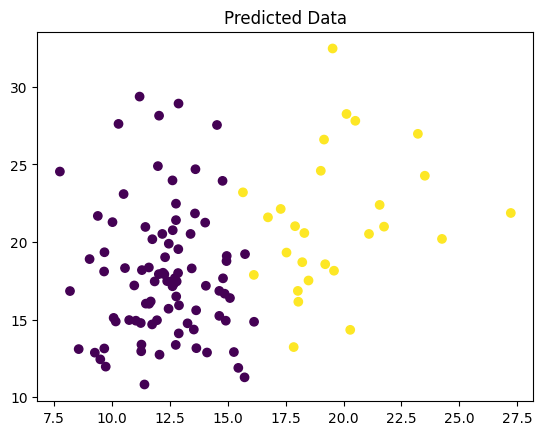
\includegraphics[width=10cm]{ch/figures/ch5.2.png}
    \caption{Scatter plot of the test data}
    \label{fig:scatter4}
\end{figure}
\begin{figure}[ht]
    \centering
    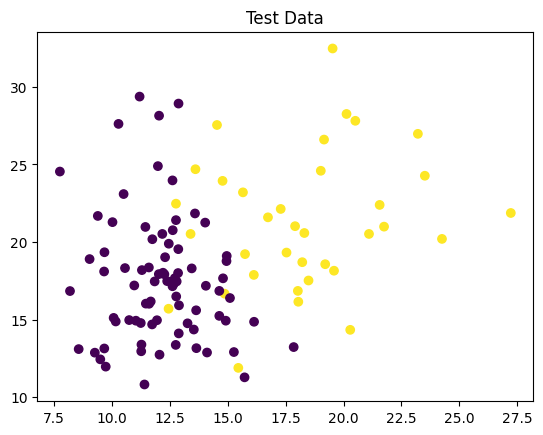
\includegraphics[width=10cm]{ch/figures/ch5.1.png}
    \caption{Scatter plot of the predicted data}
    \label{fig:scatter4}
\end{figure}
\newpage
\subsection{Confusion Matrix}
\begin{figure}[ht]
    \centering
    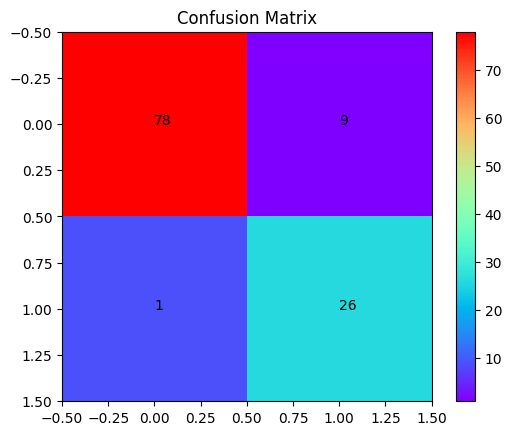
\includegraphics[width=8cm]{ch/figures/ch5.3.png}
    \caption{Confusion Matrix}
    \label{fig:loss}
\end{figure}
\newpage
\section{Design and implementation of Hopfield neural network}
\section{Introduction}
Hopfield neural network is a type of recurrent neural network. It is a form of associative memory. It is a fully connected network where each neuron is connected to every other neuron. It is a content addressable memory system with binary threshold units.\\
\section{Implementing the algorithm}
\begin{minted}{python3}
    class HopfieldNetwork:
    def __init__(self, n):
        self.n = n
        self.weights = []
        self.threshold = 0
    
    def fit(self, X):
        self.weights = np.zeros((self.n, self.n))
        for x in X:
            self.weights += np.outer(x, x)
            print(self.weights)
        # self.weights /= self.n
        np.fill_diagonal(self.weights, 0)
        self.threshold = 0
    
    def predict(self, x):
        y = np.dot(self.weights, x) - self.threshold
        y[y >= 0] = 1
        y[y < 0] = -1
        return y
\end{minted}
\subsection{Training and testing the model}
\begin{minted}{python3}
    from random import randint
    X = np.array([[1, -1, 1, -1, 1, 1, -1, 1],
                  [1, 1, 1, -1, -1, -1, 1, 1]])
    hn = HopfieldNetwork(8)
    hn.fit(X)
    pred = hn.predict([1, -1, 1, 0, 1, 1, -1, 0])
    print(f'predicted pattern: {pred}')
\end{minted}
\subsection{Output}
predicted pattern: [ 1. -1.  1. -1.  1.  1. -1.  1.]


\section{Conclusion}
In this lab, we have implemented the Kohonen Self-organizing neural network and the Hopfield neural network. We have also visualized the results of the Kohonen Self-organizing neural network.\\





